\documentclass{subfile} 


\begin{document}
  The drum pads use a piezoelectric sensor to detect vibrations, an analog circuit to 
  convert the sensor's signal to a logic level signal, and some additional processing 
  logic on the FPGA to generate the necessary signals to drive all parts of the 
  design. 

  \subsection{Physical Drum Pads} 
  The drum pads are made by glueing a piezoelectric sensor to one side of a sheet of 
  metal, and a piece of rubber to the other.
  Additionally, in order to isolate the sensor from vibrations that do not come from the 
  striking the rubber surface atop the metal, and to protect the sensor from hard surfaces 
  underneath,
  there needs to be a soft base of cloth or foam on which to put the drum pads.

  \subsection{Circuit} 
  \begin{figure}[h]
    \centering 
    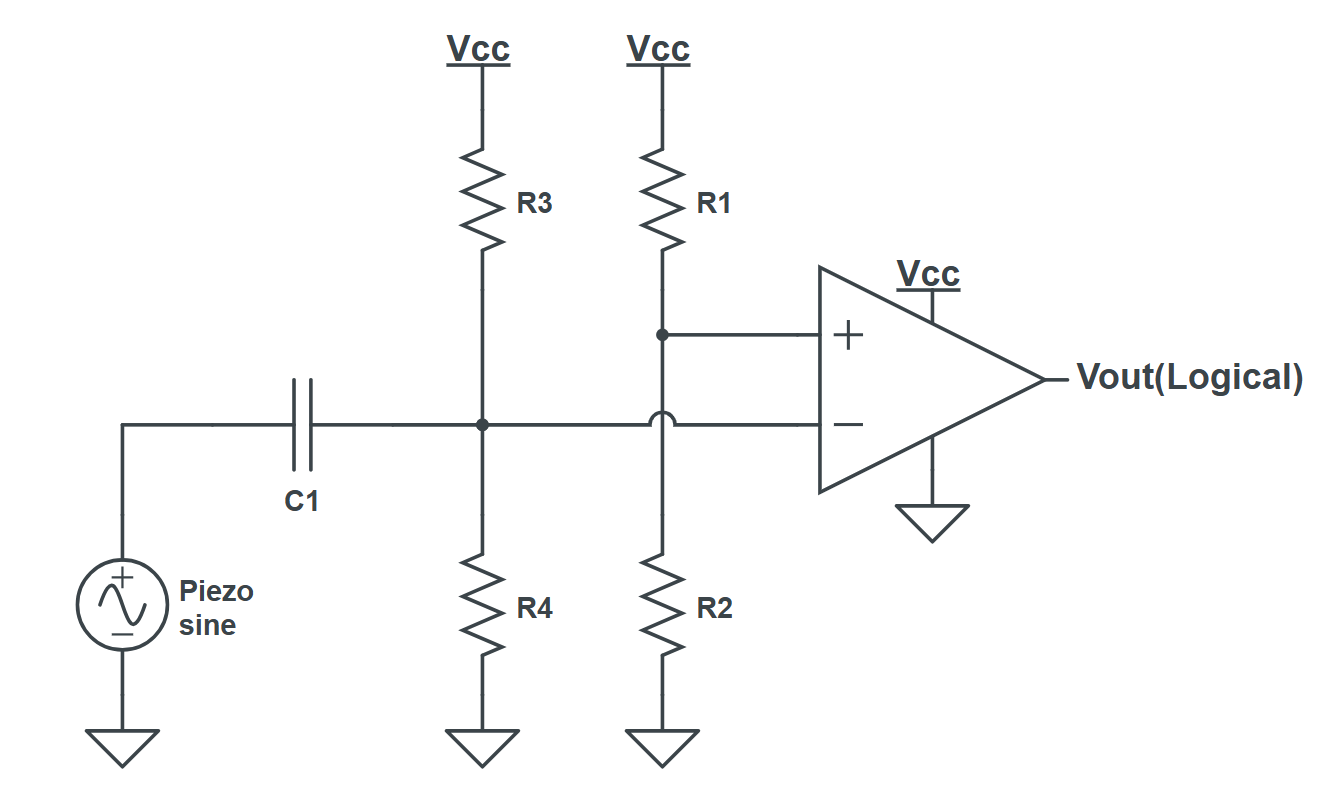
\includegraphics[width=3.5in]{piezo.png}
    \caption{Piezoelectric sensor circuit schematic} 
    \label{fig:piezo_circuit}
  \end{figure}
  A piezoelectric sensor generates an AC signal matching the vibration of the object 
  to which it is connected.
  For this application, the signal into the FPGA just had to identify when 
  the drum pad was struck, and didn't need to have any frequency or velocity information. 
  These requirements mean that the signal does not need to go through an ADC (analog to 
  digital converter), but rather 
  it can just be compared with a reference voltage to tell when the voltage across the 
  sensor reaches a certain threshold.

  The choice of this threshold was made by examining the sensor's voltage with an 
  oscilloscope, to determine what voltage would be expected by the lightest strike that 
  should be detected.

  The actual circuit is composed of an op-amp configured as an inverting comparator, with a 
  1V reference voltage, and a 3V DC bias applied to the sensor's output. 
  This effectively detects negative voltage across the sensor below -2V.

  The action of an inverting op-amp comparator circuit is fairly simple. 
  It generates an output equal to its negative supply voltage when the voltage at 
  the negative input terminal is greater than the voltage at the positive input terminal.
  When the opposite is true, the output will be equal to the positive supply voltage. 
  By providing the op-amp with 5V and ground (from the DE1-SoC board), it can detect 
  voltage differences and convert then to logic level signals appropriate for an FPGA.

  The piezoelectric sensor generates a strong negative voltage when the drum pad 
  is initially struck.
  In order to accurately detect negative voltage like this, the sensor had to be biased 
  up a few volts due to the property of op-amps where voltage at the input terminals 
  cannot go below the negative supply, which is in this case 0V.
  The biasing circuit is simply a voltage divider, and a DC-blocking capacitor between the 
  voltage divider and the sensor.
  While it may be possible to flip the sensor around in the circuit and detect a positive 
  voltage instead, this method was found to be less reliable, so the described design was 
  implemented.

  \subsection{FPGA Processing} 
  The additional processing performed in the FPGA can be likened to debouncing. 
  Due to the sensor picking up the sinusoidal vibrations within the metal of the drum pads, 
  the FPGA receives a high signal at least twice for every strike on the drum pad. 
  The FPGA must reject the secondary spikes in the signal. 
  This is done by setting starting a counter on the rising edge of the first spike, 
  and not checking for more impulses until the counter has reached some 
  interval, in this case 15 milliseconds.
  The debounced output is set to high for this 15 millisecond interval, and a one 
  clock cycle enable signal is generated when the counter starts.
  Fifteen milliseconds was chosen because the secondary spikes in the circuit's 
  output were found to end about 10 milliseconds after the initial spike.
  This latency is extremely good, as it is borderline impossible for a human to strike 
  a drum more than once in this interval.
\end{document}
